\documentclass[12pt, a4paper]{article}

%% ─── Packages ────────────────────────────────────────────────────────────────
\usepackage[utf8]{inputenc}
\usepackage[T1]{fontenc}
\usepackage[english]{babel}
\usepackage{lmodern}
\usepackage{microtype}

\usepackage[top=2.5cm, bottom=2.5cm, left=2.8cm, right=2.8cm]{geometry}

\usepackage{amsmath, amssymb}
\usepackage{mathtools}

\usepackage{booktabs}
\usepackage{array}
\usepackage{multirow}
\usepackage{xcolor}
\usepackage{colortbl}

\usepackage{graphicx}
\usepackage{float}

\usepackage[hidelinks]{hyperref}

\usepackage{fancyhdr}
\usepackage{titlesec}
\usepackage{enumitem}
\usepackage{parskip}
\usepackage{setspace}

\usepackage{algorithm}
\usepackage{algpseudocode}

%% ─── Colours ─────────────────────────────────────────────────────────────────
\definecolor{ensiie}{RGB}{30, 80, 160}
\definecolor{lightblue}{RGB}{220, 235, 255}

%% ─── Typography ──────────────────────────────────────────────────────────────
\setstretch{1.15}

\titleformat{\section}
  {\normalfont\large\bfseries}{\thesection}{1em}{}

\titleformat{\subsection}
  {\normalfont\normalsize\bfseries}{\thesubsection}{1em}{}

%% ─── Header / Footer ─────────────────────────────────────────────────────────
\pagestyle{fancy}
\fancyhf{}
\fancyhead[L]{\small\color{gray}CORO Project --- Coupe Breitling 100/24}
\fancyhead[R]{\small\color{gray}ENSIIE · 2025--2026}
\fancyfoot[C]{\thepage}
\renewcommand{\headrulewidth}{0.4pt}

%% ─── Math helpers ────────────────────────────────────────────────────────────
\newcommand{\ZZ}{\mathbb{Z}}
\newcommand{\dist}[2]{d(#1,\,#2)}

%% ═════════════════════════════════════════════════════════════════════════════
\begin{document}

%% ─── Title page ──────────────────────────────────────────────────────────────
\begin{titlepage}
\thispagestyle{empty}
\begin{center}
\vspace*{1.5cm}

{\fontsize{16pt}{20pt}\selectfont
  \textbf{\'Ecole Nationale Sup\'erieure d'Informatique\\
          pour l'Industrie et l'Entreprise}}\\[0.6cm]

\textcolor{ensiie}{\rule{\textwidth}{2pt}}\\[0.4cm]

{\large \textbf{Complements and Tools of Operations Research (CORO)}}\\[0.4cm]

{\LARGE \textbf{Aerodrome Race Optimisation}}\\[0.3cm]
{\large \textit{Inspired by the Coupe Breitling 100/24}}\\[0.5cm]

\textcolor{ensiie}{\rule{\textwidth}{2pt}}\\[1.5cm]

\begin{flushleft}
\textbf{Student} \hfill \textbf{Score} \\
\rule{\textwidth}{1pt} \\[0.2cm]
DIN Sokheng \hfill \ldots\ldots \\[0.3cm]
\rule{\textwidth}{1pt}
\end{flushleft}

\vspace{0.8cm}

\begin{flushleft}
\textbf{Lecturer:} Prof.\ Eric Soutil
\end{flushleft}

\vspace{0.5cm}
\textbf{\large Academic Year 2025--2026}

\vfill
\end{center}
\end{titlepage}

%% ─── Table of contents ───────────────────────────────────────────────────────
\tableofcontents
\newpage

%% ═════════════════════════════════════════════════════════════════════════════
\section{Introduction and Problem Statement}
%% ═════════════════════════════════════════════════════════════════════════════

This project addresses a combinatorial optimisation problem inspired by the
\textit{Coupe Breitling 100/24}, a French aeronautical competition in which pilots
fly small aircraft across France, landing at as many aerodromes as possible within
24~hours. Organisers impose geographic regions that must each be visited at least once
to ensure spatial coverage of the territory.

We are given $n$ aerodromes numbered $1,\ldots,n$. Each aerodrome~$i$ has integer
coordinates $(x_i, y_i)$ and belongs to region $r_i \in \{0,1,\ldots,m\}$, where
$r_i = 0$ means no region is assigned. We are also given a starting aerodrome~$s$,
an arriving aerodrome~$t$, a minimum number $V_{\min}$ of aerodromes to visit, and a
maximum range~$R$ (the furthest distance a plane can fly without landing).
Distances are computed as the Euclidean distance rounded to the nearest integer:
\[
  \dist{i}{j} \;=\; \mathrm{round}\!\left(\sqrt{(x_i - x_j)^2 + (y_i - y_j)^2}\right).
\]

The objective is to find a directed path $s = v_1 \to v_2 \to \cdots \to v_k = t$
minimising the total distance $\sum_{\ell=1}^{k-1} \dist{v_\ell}{v_{\ell+1}}$
subject to:
\begin{align}
  &\dist{v_\ell}{v_{\ell+1}} \leq R
    \quad \forall\,\ell = 1,\ldots,k{-}1
    && \text{(range constraint)}, \label{eq:range}\\[2pt]
  &\forall\,\kappa \in \{1,\ldots,m\},\;\;
    \exists\,\ell : r_{v_\ell} = \kappa
    && \text{(region coverage)}, \label{eq:cover}\\[2pt]
  &k \geq V_{\min}
    && \text{(minimum visits)}. \label{eq:card}
\end{align}

This problem is related to the Travelling Salesman Problem (TSP) studied in the
lectures, but differs in several important ways. First, we seek a \emph{path} from $s$
to $t$, not a Hamiltonian cycle. Second, we select a \emph{subset} of aerodromes to
visit rather than visiting all of them. Third, the region-covering
constraints~\eqref{eq:cover} impose a set-covering structure that has no direct
analogue in the classical TSP. Finally, the range constraint~\eqref{eq:range}
restricts which consecutive pairs are feasible, unlike the complete graph assumption
in standard TSP.

\subsection{Graph Construction}

We construct a directed graph $G = (V, A)$ where $V = \{1,\ldots,n\}$ and
$A = \{(i,j) : i \neq j,\;\dist{i}{j} \leq R\}$.
The range constraint~\eqref{eq:range} is enforced structurally: arcs violating it
simply do not exist. This reduces the number of binary variables from $n(n{-}1)$ to
$|A|$, which can be significantly smaller when $R$ is tight relative to the
coordinate domain.


%% ═════════════════════════════════════════════════════════════════════════════
\section{ILP Model~1: MTZ Formulation}
%% ═════════════════════════════════════════════════════════════════════════════

The first model uses the Miller--Tucker--Zemlin (MTZ) subtour elimination
technique~\cite{mtz}, which was presented in the lectures in the context of
the asymmetric TSP. The idea is to introduce continuous \emph{position} variables
$u_i$ that assign each visited node its order along the path; a subtour is
impossible because positions must strictly increase along any sequence of used arcs.

\subsection{Variables}

\begin{itemize}[nosep]
  \item $x_{ij} \in \{0,1\}$ for each $(i,j) \in A$: arc $(i,j)$ is in the path.
  \item $y_i \in \{0,1\}$ for each $i \in V$: aerodrome $i$ is visited.
  \item $u_i \in [0,\,n]$ for each $i \in V$: position of $i$ along the path
        (continuous).
\end{itemize}

\subsection{Objective}

\[
  \min \sum_{(i,j) \in A} \dist{i}{j}\; x_{ij}.
\]

\subsection{Constraints}

\paragraph{(C1) Source flow.}
The path starts at $s$: exactly one arc leaves $s$, none enters it.
\[
  \sum_{j:(s,j)\in A} x_{sj} = 1, \qquad
  \sum_{j:(j,s)\in A} x_{js} = 0.
\]

\paragraph{(C2) Sink flow.}
The path ends at $t$: exactly one arc enters $t$, none leaves it.
\[
  \sum_{j:(j,t)\in A} x_{jt} = 1, \qquad
  \sum_{j:(t,j)\in A} x_{tj} = 0.
\]

\paragraph{(C3) Flow balance at intermediate nodes.}
For every $i \in V \setminus \{s,t\}$:
\[
  \sum_{j:(j,i)\in A} x_{ji} = y_i, \qquad
  \sum_{j:(i,j)\in A} x_{ij} = y_i.
\]
A node is visited ($y_i = 1$) if and only if exactly one arc enters it and one
leaves it. If $y_i = 0$, no arc touches node~$i$.

\paragraph{(C4) Endpoints visited.}
$y_s = 1$, $\;y_t = 1$.

\paragraph{(C5) Region coverage.}
For each region $\kappa = 1,\ldots,m$:
\[
  \sum_{i:\,r_i = \kappa} y_i \;\geq\; 1.
\]
This is a classical \emph{set covering} constraint: at least one aerodrome from each
region must be selected.

\paragraph{(C6) Minimum visits.}
$\displaystyle\sum_{i \in V} y_i \;\geq\; V_{\min}.$

\paragraph{(C7) MTZ subtour elimination.}
For all $(i,j) \in A$ with $i \neq s$ and $j \neq s$:
\[
  u_i - u_j + n\,x_{ij} \;\leq\; n - 1.
\]

This is the core of the MTZ formulation. We analyse the two cases:
\begin{itemize}[nosep]
  \item If $x_{ij} = 0$: the constraint becomes $u_i - u_j \leq n-1$, which is
        always satisfied since $u_i \leq n$ and $u_j \geq 0$. The constraint is
        inactive.
  \item If $x_{ij} = 1$: the constraint becomes $u_j \geq u_i + 1$. This forces
        node~$j$ to have a strictly later position than node~$i$ in the path.
\end{itemize}
Since positions strictly increase along every used arc, any subset of nodes forming
a directed cycle would require positions to simultaneously increase and return to
their starting value, which is impossible. This eliminates all subtours.

As discussed in the lectures on the TSP, the MTZ formulation uses only
$O(n^2)$ constraints (polynomial), but its LP relaxation is weaker than the subtour
polytope because the continuous $u_i$ variables allow fractional solutions that
``look like'' subtours to the relaxation. This typically leads to more
branch-and-bound nodes compared to the SEC formulation.

\paragraph{(C8) Linking position to visit.}
$u_s = 0$, and for all $i \neq s$: $u_i \leq n \cdot y_i$.

If node $i$ is not visited ($y_i = 0$), this forces $u_i = 0$, which tightens the
LP relaxation by preventing unvisited nodes from taking arbitrary position values.

\subsection{MTZ Algorithm Overview}

The model is passed to HiGHS, which solves it via branch-and-bound. The pseudocode
below summarises the overall resolution procedure.

\begin{algorithm}[H]
\caption{MTZ-based solve}
\begin{algorithmic}[1]
\State Build arc set $A = \{(i,j) : \dist{i}{j} \leq R,\; i \neq j\}$.
\State Formulate ILP with variables $x_{ij}$, $y_i$, $u_i$ and constraints (C1)--(C8).
\State Solve LP relaxation at root $\Rightarrow$ lower bound $z_{\mathrm{LP}}$.
\If{LP solution is integer}
  \State \Return LP solution.
\EndIf
\State Branch on a fractional $x_{ij}$ variable (set to 0 or 1).
\Repeat
  \State Solve LP at current B\&B node.
  \If{LP infeasible} \textbf{prune} (infeasibility). \EndIf
  \If{LP bound $\geq$ incumbent $z^*$} \textbf{prune} (bound). \EndIf
  \If{LP solution is integer and cost $< z^*$} update $z^* \leftarrow$ cost. \EndIf
  \State Otherwise, branch on the most fractional variable.
\Until{B\&B queue is empty}
\State \Return best integer solution found with cost $z^*$.
\end{algorithmic}
\end{algorithm}


%% ═════════════════════════════════════════════════════════════════════════════
\section{ILP Model~2: Subtour Elimination Constraints (SEC)}
%% ═════════════════════════════════════════════════════════════════════════════

The second model replaces the MTZ constraints with \emph{subtour elimination
constraints} (SEC), following the approach of Dantzig, Fulkerson, and
Johnson~\cite{dantzig}. This was also covered in the lectures as the
stronger formulation for the TSP, where we saw that SEC describes the subtour
polytope exactly and yields a tighter LP relaxation than MTZ.

\subsection{Variables and Base Constraints}

The model uses the same $x_{ij}$ and $y_i$ variables and the same constraints
(C1)--(C6) as Model~1. The position variables $u_i$ and constraints (C7)--(C8) are
removed entirely.

\subsection{Subtour Elimination}

For every non-empty subset $S \subseteq V \setminus \{s,t\}$:
\begin{equation}\label{eq:sec}
  \sum_{\substack{(i,j) \in A \\ i \in S,\; j \in S}} x_{ij}
  \;\leq\; |S| - 1.
  \tag{SEC}
\end{equation}

The reasoning is combinatorial: among $|S|$ nodes, any acyclic subgraph (in
particular, a forest) can use at most $|S|-1$ arcs. If the number of arcs within $S$
reaches $|S|$ or more, a directed cycle must exist within $S$. Since such a cycle
would be disconnected from the $s$--$t$ path (because $s,t \notin S$), the
constraint forbids it.

The number of possible subsets $S$ is $2^{n-2}$, so we cannot add all constraints
upfront. This is the same situation encountered in the lectures on cutting
plane methods: we have an exponential family of valid inequalities and must use a
\emph{separation procedure} to identify violated ones on the fly.

\subsection{Iterative Solve-and-Cut}

Our implementation uses the following iterative approach, which is a simplified
version of the cutting plane algorithm from the lectures on Gomory cuts and
SEC for the TSP:

\begin{algorithm}[H]
\caption{Iterative SEC generation}
\begin{algorithmic}[1]
\State Solve the ILP with constraints (C1)--(C6) only.
\Loop
  \State Extract the integer solution. Build the subgraph of arcs with $x_{ij} = 1$.
  \State BFS from $s$: find all nodes reachable from $s$ along used arcs.
  \State Let $U \leftarrow \{i \in V : y_i = 1 \text{ and } i \text{ not reachable
         from } s\}$.
  \If{$U = \emptyset$}
    \State \Return current solution --- it is a valid $s$--$t$ path.
  \EndIf
  \For{each connected component $S$ of the subgraph restricted to $U$}
    \State Add: $\displaystyle\sum_{(i,j) \in A,\, i \in S,\, j \in S}
           x_{ij} \leq |S| - 1$.
  \EndFor
  \State Re-solve the ILP with the additional constraints.
\EndLoop
\end{algorithmic}
\end{algorithm}

The \textbf{separation procedure} here is simple: given an integer solution, find
connected components among visited nodes not reachable from $s$. Each such component
is a subtour, and we add one SEC constraint per component. This runs in $O(n + |A|)$
time using BFS or DFS.

In the lectures, we also discussed a more sophisticated approach:
\emph{lazy constraint callbacks}, where the solver calls the separation procedure at
each integer-feasible node during its own branch-and-bound, without restarting the
entire solve. Our iterative implementation is simpler but slower, because each
re-solve discards the branch-and-bound tree from the previous iteration.

\subsection{Why SEC gives a tighter LP relaxation}

The LP relaxation of the SEC formulation describes the \emph{subtour polytope}, which
is a tighter outer approximation of the integer hull than the MTZ LP relaxation. In
the notation from the lectures on LP duality and relaxation quality:
\[
  z_{\mathrm{LP}}^{\mathrm{SEC}} \;\geq\; z_{\mathrm{LP}}^{\mathrm{MTZ}}
  \;\geq\; z_{\mathrm{ILP}}^*.
\]
A tighter LP bound means the branch-and-bound algorithm can prune more nodes (by the
bound criterion from the B\&B lecture: prune when the LP bound of a node is worse than
the best known incumbent), so fewer nodes are typically explored.


%% ═════════════════════════════════════════════════════════════════════════════
\section{Heuristic}
%% ═════════════════════════════════════════════════════════════════════════════

Since exact methods may time out on large instances, we designed a heuristic with
three phases: greedy construction~\cite{nn_heuristic}, 2-opt local
search~\cite{lin2opt}, and node removal~\cite{lk}.

\subsection{Phase~1: Greedy Construction}

Starting from $s$, the algorithm builds a path by iteratively choosing the next node
using a nearest-neighbour strategy with region-coverage priority.

\begin{algorithm}[H]
\caption{Greedy construction}
\begin{algorithmic}[1]
\State $\text{path} \leftarrow [s]$;\quad $\text{visited} \leftarrow \{s\}$;\quad $\text{covered} \leftarrow \{r_s\} \setminus \{0\}$;\quad $v \leftarrow s$
\While{$|\text{covered}| < m$ \textbf{or} $|\text{visited}| < V_{\min}$}
  \State $N \leftarrow \{j \notin \text{visited} : \dist{v}{j} \leq R\}$
  \If{$N = \emptyset$}
    \State Dijkstra escape: find shortest range-feasible path from $v$ to any new node, append it.
    \State \textbf{break} if still stuck.
  \EndIf
  \State $N_{\text{unc}} \leftarrow \{j \in N : r_j > 0 \text{ and } r_j \notin \text{covered}\}$
  \State $\text{next} \leftarrow \arg\min_{j \in N_{\text{unc}}} \dist{v}{j}$ \quad if $N_{\text{unc}} \neq \emptyset$, \quad else $\arg\min_{j \in N} \dist{v}{j}$
  \State Append $\text{next}$ to path; update visited and covered.
  \State $v \leftarrow \text{next}$
\EndWhile
\If{$v \neq t$}
  \State If $\dist{v}{t} \leq R$: append $t$.
  \State Else: append shortest Dijkstra path from $v$ to $t$.
\EndIf
\end{algorithmic}
\end{algorithm}

The greedy nearest-neighbour strategy follows Rosenkrantz, Stearns and
Lewis~\cite{nn_heuristic}, who showed it achieves a $O(\log n)$ approximation ratio
for metric TSP. Here it is extended with region-coverage priority.
Its time complexity is $O(n^2)$.

\subsection{Phase~2: 2-opt Local Search}

Given the path $P = [v_1, v_2, \ldots, v_k]$, the 2-opt procedure tests reversing
every interior segment until no improvement is found.

\begin{algorithm}[H]
\caption{2-opt local search}
\begin{algorithmic}[1]
\Repeat
  \State $\text{improved} \leftarrow \text{false}$
  \For{$i = 2$ \textbf{to} $k-2$}
    \For{$j = i+1$ \textbf{to} $k-1$}
      \State Reverse segment: $P' \leftarrow [v_1,\ldots,v_{i-1},v_j,v_{j-1},\ldots,v_i,v_{j+1},\ldots,v_k]$
      \If{all consecutive pairs in $P'$ satisfy $d \leq R$ \textbf{and} $\text{cost}(P') < \text{cost}(P)$}
        \State $P \leftarrow P'$;\quad $\text{improved} \leftarrow \text{true}$
      \EndIf
    \EndFor
  \EndFor
\Until{$\neg\,\text{improved}$}
\end{algorithmic}
\end{algorithm}

The 2-opt move was introduced by Lin~\cite{lin2opt} and remains one of the most
effective local search improvements for routing problems.
Each pass is $O(k^2)$; the range check also verifies all pairs within the reversed segment.

\subsection{Phase~3: Node Removal}

After 2-opt, we attempt to shorten the path by removing unnecessary interior nodes.
This greedy node-removal step is in the spirit of the Lin--Kernighan
framework~\cite{lk}, which systematically removes edges to find cheaper
reconnections.

\begin{algorithm}[H]
\caption{Node removal}
\begin{algorithmic}[1]
\Repeat
  \State $\text{best\_save} \leftarrow 0$;\quad $\text{best\_idx} \leftarrow -1$
  \For{$\ell = 2$ \textbf{to} $k-1$}
    \If{$\dist{v_{\ell-1}}{v_{\ell+1}} \leq R$
        \textbf{and} $|\text{path}|-1 \geq V_{\min}$
        \textbf{and} region $r_{v_\ell}$ covered by another visited node}
      \State $\text{save} \leftarrow \dist{v_{\ell-1}}{v_\ell} + \dist{v_\ell}{v_{\ell+1}} - \dist{v_{\ell-1}}{v_{\ell+1}}$
      \If{$\text{save} > \text{best\_save}$}
        \State $\text{best\_save} \leftarrow \text{save}$;\quad $\text{best\_idx} \leftarrow \ell$
      \EndIf
    \EndIf
  \EndFor
  \If{$\text{best\_idx} \neq -1$}
    \State Remove $v_{\text{best\_idx}}$ from path.
  \EndIf
\Until{$\text{best\_idx} = -1$}
\end{algorithmic}
\end{algorithm}


%% ═════════════════════════════════════════════════════════════════════════════
\section{Computational Results}
%% ═════════════════════════════════════════════════════════════════════════════

All experiments used the HiGHS solver~\cite{highs} via JuMP~\cite{jump} in Julia,
with a \textbf{120\,s time limit} per ILP solve. We report results on the three
provided instances.

\subsection{Instance \texttt{instance\_6\_1} ($n=6$, $m=2$, $R=6$, $V_{\min}=4$)}

The range graph has 24~feasible arcs.

\begin{table}[H]
\centering
\caption{Results on \texttt{instance\_6\_1}.}
\begin{tabular}{lrrlrr}
\toprule
Method & Objective & Stops & Status & Time (s) & B\&B nodes \\
\midrule
MTZ       & \textbf{12} & 4 & OPTIMAL  & 0.09 & 1 \\
SEC       & \textbf{12} & 4 & OPTIMAL  & 0.03 & 1 \\
Heuristic & \textbf{12} & 4 & Feasible & 0.12 & --- \\
\bottomrule
\end{tabular}
\end{table}

All three methods find the optimal path $1 \to 3 \to 2 \to 5$ with cost~12. Both ILP
models solve at the root node (1~B\&B node = no branching needed). The SEC model
added 3~cuts before converging.

\begin{figure}[H]
  \centering
  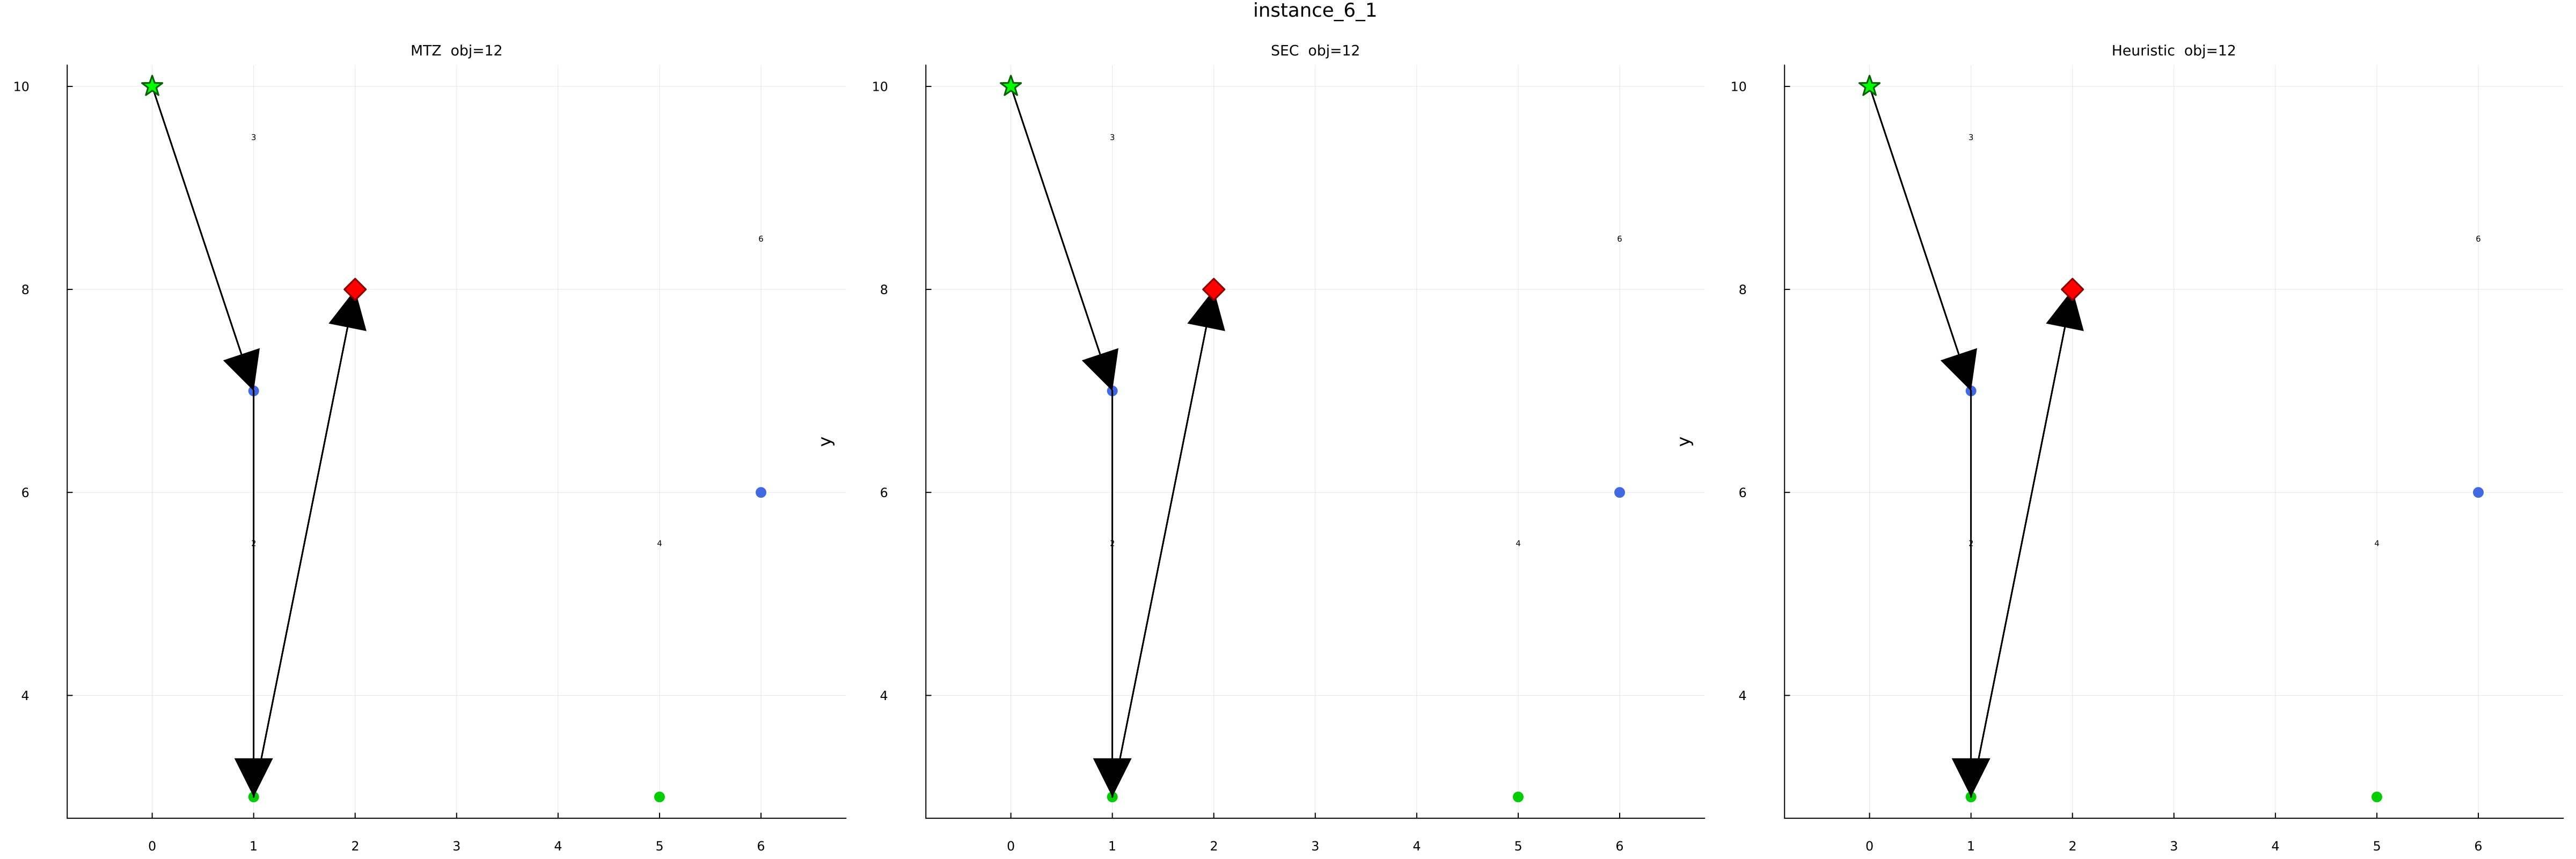
\includegraphics[width=\textwidth]{instance_6_1_results.png}
  \caption{Solution paths on \texttt{instance\_6\_1}. Green star~$= s$,
           red diamond~$= t$, colours indicate regions.}
\end{figure}

\subsection{Instance \texttt{instance\_40\_1} ($n=40$, $m=2$, $R=26$, $V_{\min}=14$)}

The range graph has 420~feasible arcs.

\begin{table}[H]
\centering
\caption{Results on \texttt{instance\_40\_1}.}
\begin{tabular}{lrrlrr}
\toprule
Method & Objective & Stops & Status & Time (s) & B\&B nodes \\
\midrule
MTZ       & \textbf{114} & 14 & OPTIMAL   & 4.63   & 1\,295 \\
SEC       & \textbf{114} & 14 & OPTIMAL   & 35.29  & 35 \\
Heuristic & 149          & 13$^\dagger$ & Invalid$^\dagger$ & $<$0.01 & --- \\
\bottomrule
\end{tabular}
\end{table}
{\small $^\dagger$\,Heuristic produced an invalid solution: only 13~distinct stops
($< V_{\min} = 14$) and the path contains a duplicated node.}

\medskip

Both ILP models prove the optimal cost of~114 with path
$27 \to 7 \to 10 \to 23 \to 11 \to 32 \to 3 \to 4 \to 9 \to 28 \to 22 \to 24
\to 35 \to 8$.

MTZ is $\approx 8\times$ faster despite exploring $37\times$ more B\&B nodes
(1\,295 vs.~35). This counter-intuitive result is explained by the overhead of the
iterative SEC approach: the model was re-solved from scratch after adding each batch
of cuts (66~cuts total across multiple iterations), discarding the B\&B tree each
time. With lazy callbacks, the tighter LP bound of SEC would translate directly into
less total work.

\begin{figure}[H]
  \centering
  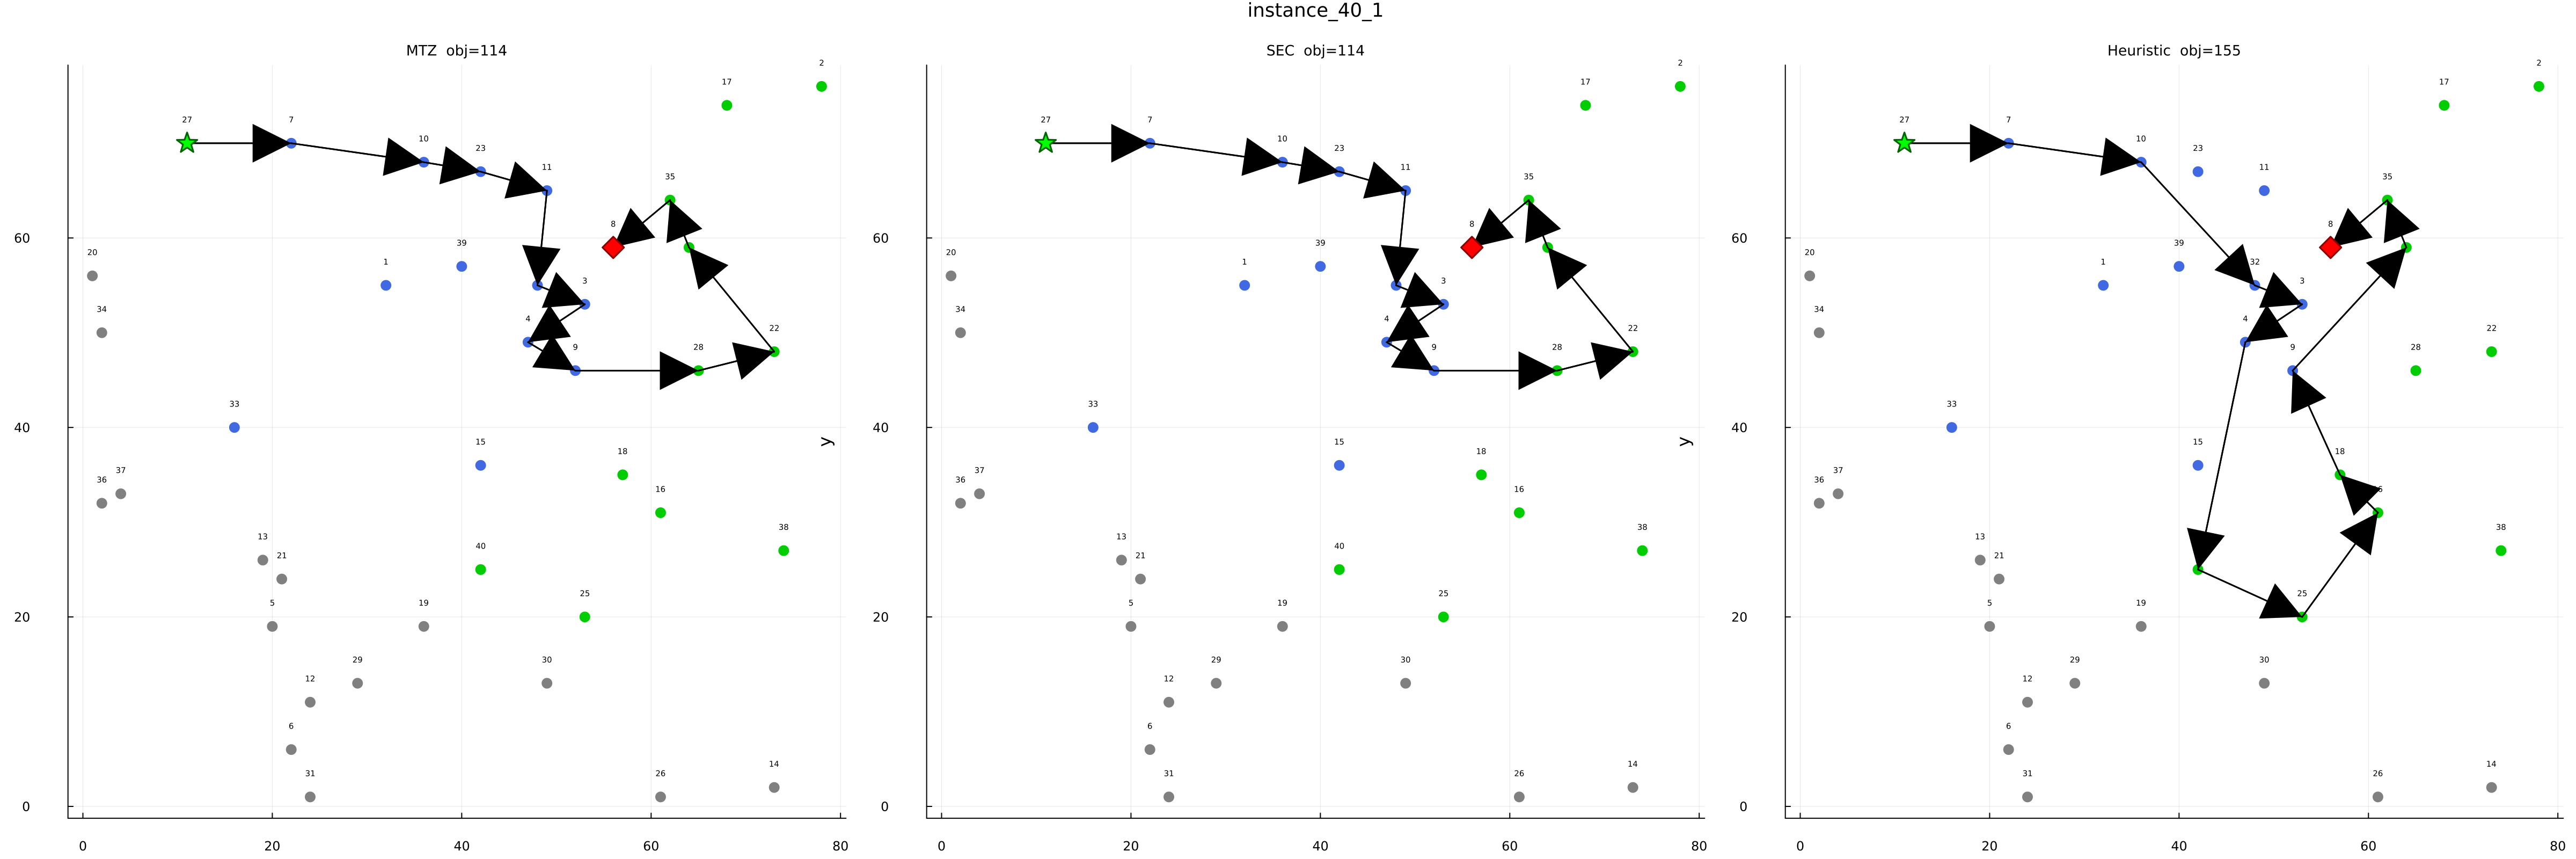
\includegraphics[width=\textwidth]{instance_40_1_results.png}
  \caption{Solution paths on \texttt{instance\_40\_1}.}
\end{figure}

\subsection{Instance \texttt{instance\_80\_1} ($n=80$, $m=9$, $R=31$, $V_{\min}=35$)}

The range graph has 614~feasible arcs.

\begin{table}[H]
\centering
\caption{Results on \texttt{instance\_80\_1}.}
\begin{tabular}{lrrlrr}
\toprule
Method & Objective & Stops & Status & Time (s) & B\&B nodes \\
\midrule
MTZ       & 948  & 49 & Time limit & 120.01 & 53\,334 \\
SEC       & ---  & ---  & Time limit & 165.41 & 13\,739 \\
Heuristic & 637  & 36 & Invalid$^\dagger$ & $<$0.01 & --- \\
\bottomrule
\end{tabular}
\end{table}
{\small $^\dagger$\,Heuristic solution contains a leg exceeding range $R=31$
(leg $19 \to 55$, dist\,=\,56).}

\medskip

Both ILP models hit the time limit. MTZ found an incumbent of cost~948
(49~stops) but could not prove optimality after 53\,334~B\&B nodes. Using the
terminology from the lecture on branch-and-bound, the tree was not fully
explored: many open nodes remained with LP bounds that could not be pruned against
the incumbent.

The SEC model explored only 13\,739~B\&B nodes (versus 53\,334 for MTZ), confirming
the tighter LP bound, but added 105~cuts across multiple iterations. Each re-solve
consumed part of the time budget, and no valid subtour-free solution was found within
165\,s.

The heuristic returns cost~637 in under 1\,ms. It visits 36 distinct nodes
($\geq V_{\min} = 35$) but contains one infeasible leg ($\dist{19}{55} = 56 > R = 31$),
producing an invalid path. This illustrates the difficulty of maintaining range
feasibility in the greedy construction when the graph is sparse.

\begin{figure}[H]
  \centering
  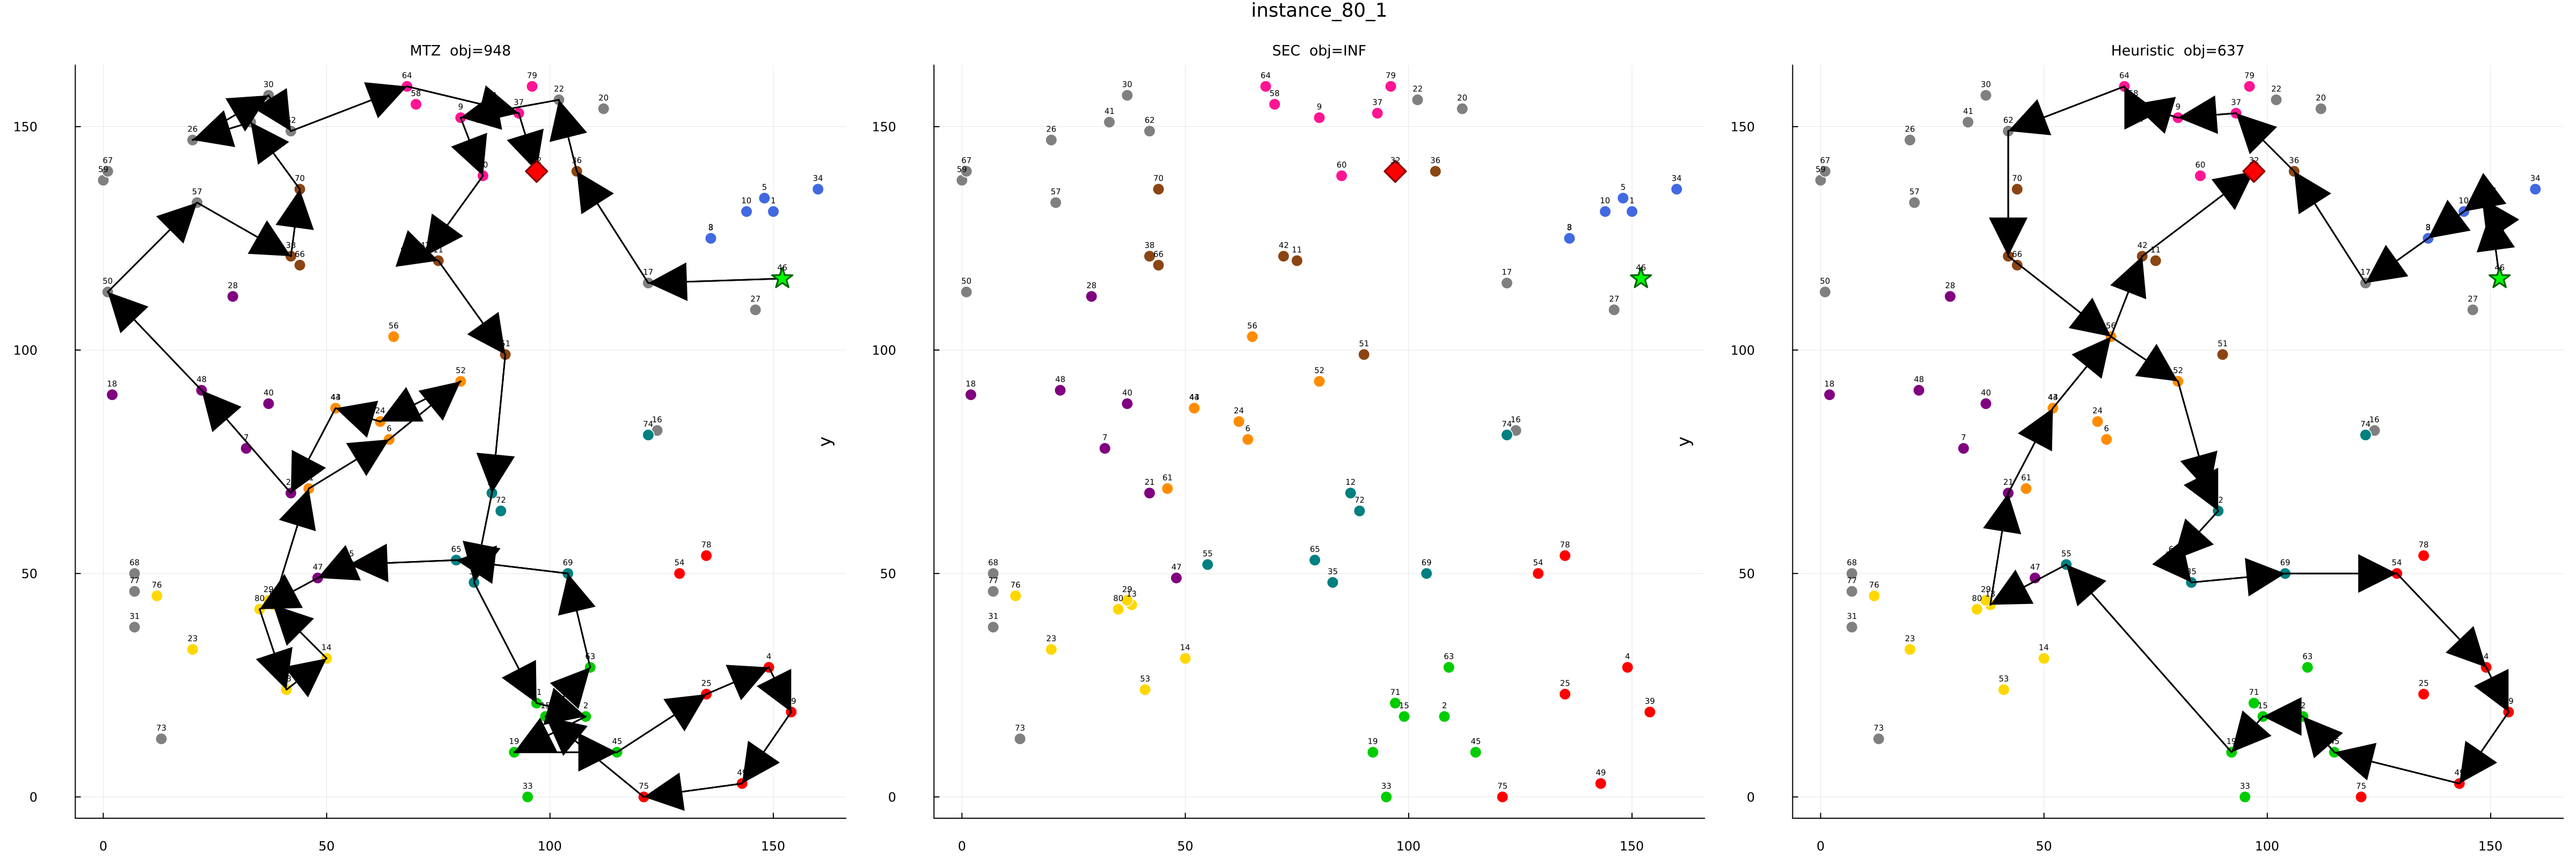
\includegraphics[width=\textwidth]{instance_80_1_results.png}
  \caption{Solution paths on \texttt{instance\_80\_1}. MTZ shows its best incumbent.
           SEC did not produce a valid path within the time limit.}
\end{figure}


\subsection{Summary}

\begin{table}[H]
\centering
\caption{Cross-instance comparison.}
\begin{tabular}{llrrrl}
\toprule
Instance & Method & Objective & Stops & Time (s) & Remark \\
\midrule
\multirow{3}{*}{\texttt{6\_1}}
  & MTZ       & 12  & 4  & 0.09    & Optimal \\
  & SEC       & 12  & 4  & 0.03    & Optimal, 3 cuts \\
  & Heuristic & 12  & 4  & 0.12    & Matches optimal \\
\midrule
\multirow{3}{*}{\texttt{40\_1}}
  & MTZ       & 114 & 14 & 4.63    & Optimal, 1\,295 nodes \\
  & SEC       & 114 & 14 & 35.29   & Optimal, 35 nodes, 66 cuts \\
  & Heuristic & 149 & 13 & $<$0.01 & Invalid ($V_{\min}$ violated) \\
\midrule
\multirow{3}{*}{\texttt{80\_1}}
  & MTZ       & 948 & 49 & 120.01  & Time limit, 53\,334 nodes \\
  & SEC       & --- & ---  & 165.41  & Time limit, 105 cuts \\
  & Heuristic & 637 & 36 & $<$0.01 & Invalid (range violated) \\
\bottomrule
\end{tabular}
\end{table}


%% ═════════════════════════════════════════════════════════════════════════════
\section{Custom Instances}
%% ═════════════════════════════════════════════════════════════════════════════

To further stress-test the models we ran seven additional instances of varying sizes.
Table~\ref{tab:custom_params} summarises their parameters and
Table~\ref{tab:custom_results} reports the computational results.

\begin{table}[H]
\centering
\caption{Custom instance parameters.}
\label{tab:custom_params}
\begin{tabular}{lrrrrrrr}
\toprule
Instance & $n$ & $m$ & $R$ & $V_{\min}$ & $s$ & $t$ & Arcs \\
\midrule
\texttt{instance\_20\_1} & 20 & 3 & 50 & 8  & 19 & 10 & 312 \\
\texttt{instance\_20\_2} & 20 & 3 & 50 & 8  &  1 & 10 & 312 \\
\texttt{instance\_20\_3} & 20 & 3 & 25 & 8  &  1 & 10 & 126 \\
\texttt{instance\_20\_4} & 20 & 3 & 40 & 8  &  1 & 15 & 246 \\
\texttt{instance\_30\_1} & 30 & 3 & 18 & 14 & 19 & 10 & 160 \\
\texttt{instance\_50\_1} & 50 & 4 & 28 & 16 & 49 & 34 & 442 \\
\texttt{instance\_70\_1} & 70 & 16 & 35 & 22 & 47 & 23 & 736 \\
\bottomrule
\end{tabular}
\end{table}

\begin{table}[H]
\centering
\caption{Results on custom instances (120\,s time limit per ILP solve).}
\label{tab:custom_results}
\begin{tabular}{llrrlrrl}
\toprule
Instance & Method & Obj. & Stops & Status & Time (s) & B\&B nodes & SEC cuts \\
\midrule
\multirow{3}{*}{\texttt{20\_1}}
  & MTZ       & \textbf{124} & 8 & Optimal   &  92.95 & 115\,901 & --- \\
  & SEC       & ---          & --- & Time lim &121.17  &      177 & 116 \\
  & Heuristic & 138          & 8 & Feasible  &   0.12 & ---      & --- \\
\midrule
\multirow{3}{*}{\texttt{20\_2}}
  & MTZ       & \textbf{104} & 8 & Optimal   &   3.33 &   1\,495 & --- \\
  & SEC       & ---          & --- & Time lim &121.79  &      224 & 120 \\
  & Heuristic & 119          & 8 & Feasible  &  $<$0.01 & ---    & --- \\
\midrule
\multirow{3}{*}{\texttt{20\_3}}
  & MTZ       & \textbf{104} & 8  & Optimal  &   1.99 &      892 & --- \\
  & SEC       & \textbf{104} & 8  & Optimal  &  51.62 &      140 & 101 \\
  & Heuristic & 117          & 8  & Feasible &  $<$0.01 & ---    & --- \\
\midrule
\multirow{3}{*}{\texttt{20\_4}}
  & MTZ       & \textbf{109} & 8 & Optimal   & 105.87 & 142\,906 & --- \\
  & SEC       & ---          & --- & Time lim &121.13  &      379 & 124 \\
  & Heuristic & 118          & 8 & Feasible  &  $<$0.01 & ---    & --- \\
\midrule
\multirow{3}{*}{\texttt{30\_1}}
  & MTZ       & \textbf{144} & 14 & Optimal  & 112.79 & 118\,915 & --- \\
  & SEC       & ---          & --- & Time lim &120.59  &    1\,100 & 134 \\
  & Heuristic & 152          & 14 & Feasible &  $<$0.01 & ---    & --- \\
\midrule
\multirow{3}{*}{\texttt{50\_1}}
  & MTZ       & \textbf{168} & 16 & Optimal  &  69.55 &  31\,175 & --- \\
  & SEC       & ---          & --- & Time lim &123.65  &      901 & 90 \\
  & Heuristic & 275$^\dagger$ & --- & Invalid &  $<$0.01 & ---    & --- \\
\midrule
\multirow{3}{*}{\texttt{70\_1}}
  & MTZ       & 469 & 22 & Time lim  & 120.02 &  32\,330 & --- \\
  & SEC       & --- & --- & Time lim & 141.22 &  11\,647 & 127 \\
  & Heuristic & 800$^\dagger$ & --- & Invalid &  $<$0.01 & ---    & --- \\
\bottomrule
\end{tabular}
\end{table}
{\small $^\dagger$\,Heuristic path contains legs exceeding range $R$ on \texttt{50\_1} and \texttt{70\_1}.}

\medskip

\paragraph{Key observations.}

\begin{itemize}[nosep]
  \item MTZ proved optimality on 5 out of 7 custom instances within the time limit,
        while SEC proved optimality only on \texttt{instance\_20\_3} (the smallest
        range graph, 126~arcs). The iterative re-solve overhead penalises SEC heavily
        when many cuts are needed.

  \item SEC consistently explores far fewer B\&B nodes than MTZ (e.g., 140 vs.\ 892
        on \texttt{20\_3}; 379 vs.\ 142\,906 on \texttt{20\_4}), confirming the
        tighter LP relaxation predicted by theory. The wall-clock disadvantage is
        entirely due to re-solve overhead.

  \item The heuristic gap on feasible solutions ranged from $+5.6\%$ (\texttt{30\_1})
        to $+14.4\%$ (\texttt{20\_2}), which is reasonable for a greedy nearest-neighbour
        approach. The heuristic failed on \texttt{50\_1} and \texttt{70\_1} due to
        range constraint violations in the greedy construction.

  \item On \texttt{instance\_70\_1} ($m = 16$ regions), neither ILP model solved
        within the time limit. MTZ found an incumbent of 469 after 120\,s; SEC added
        127~cuts but found no valid solution.
\end{itemize}

\begin{figure}[H]
  \centering
  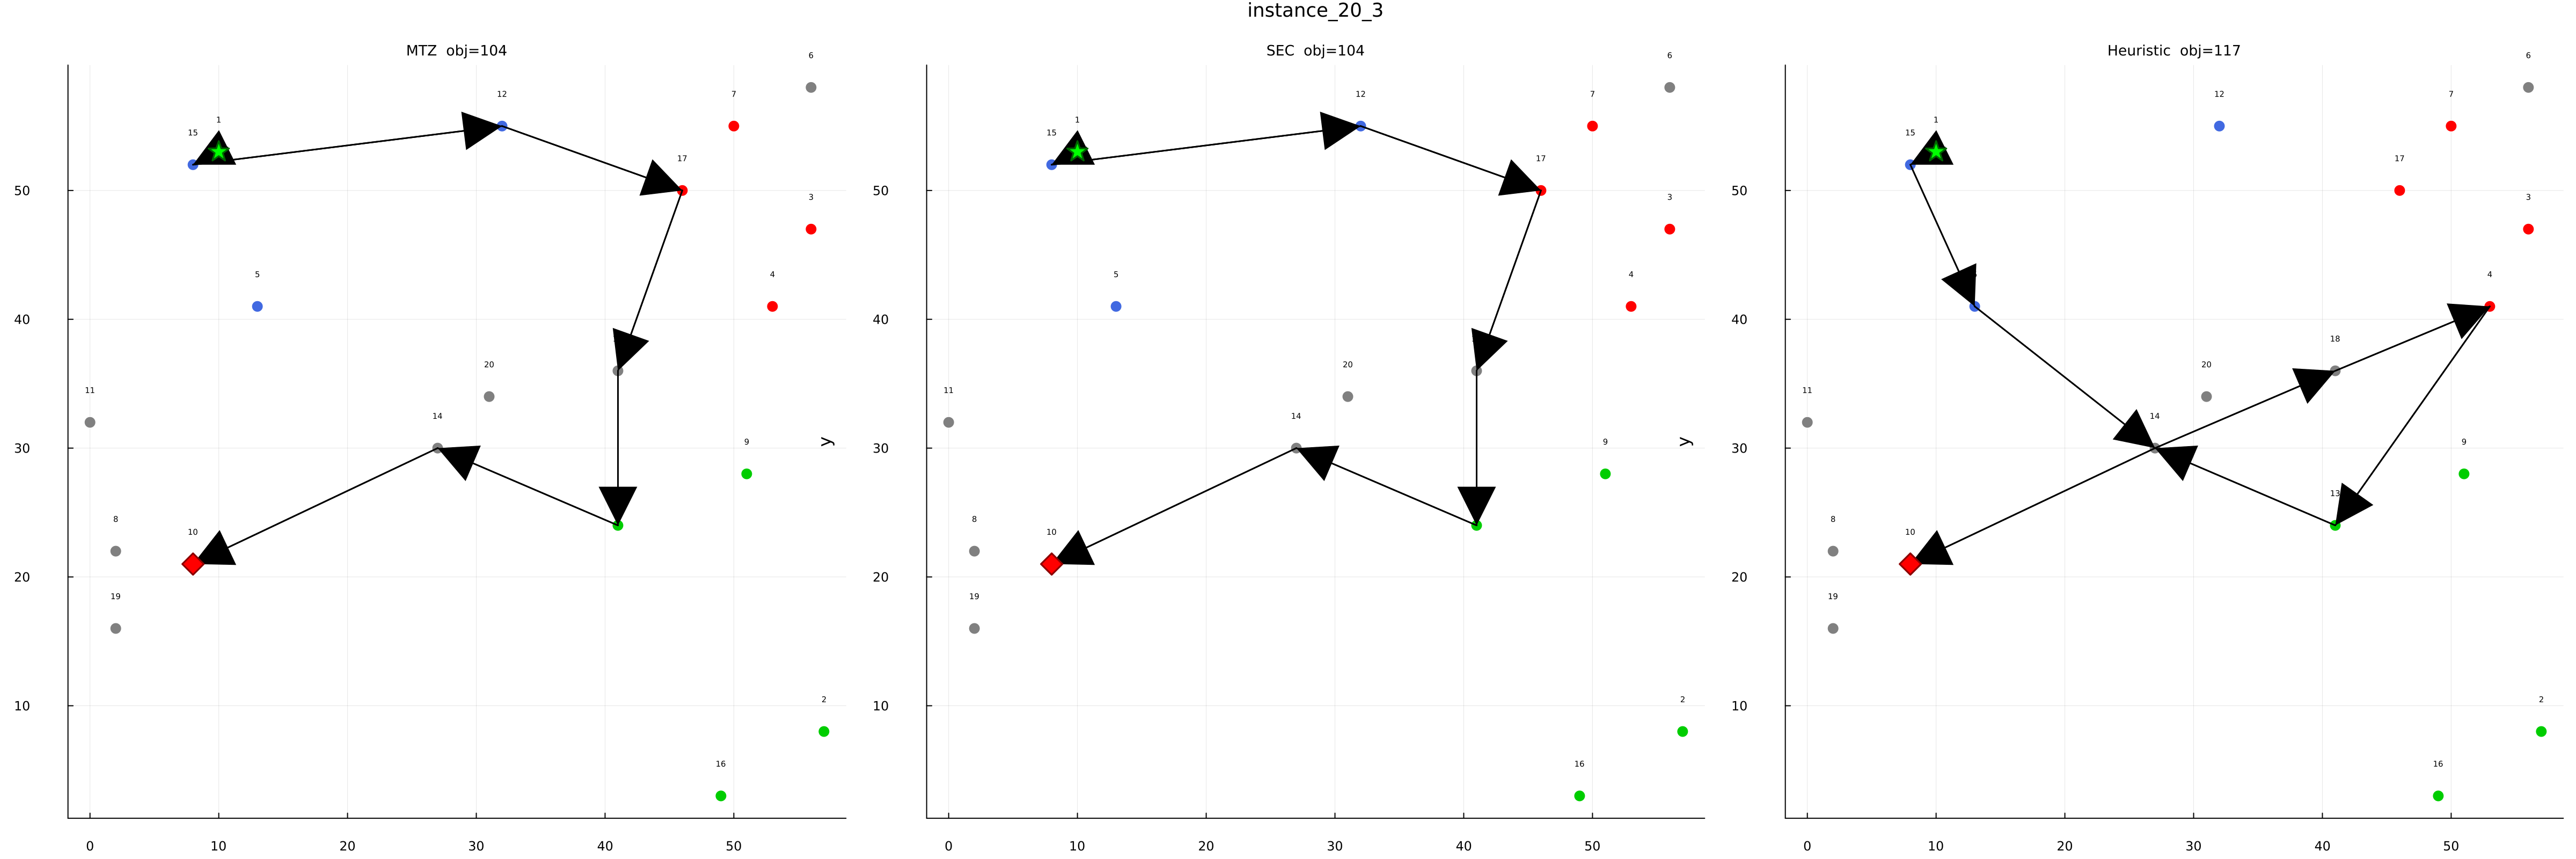
\includegraphics[width=\textwidth]{instance_20_3_results.png}
  \caption{Solution paths on \texttt{instance\_20\_3} --- the only custom instance
           where both ILP models found the optimum (cost~104).}
\end{figure}

\begin{figure}[H]
  \centering
  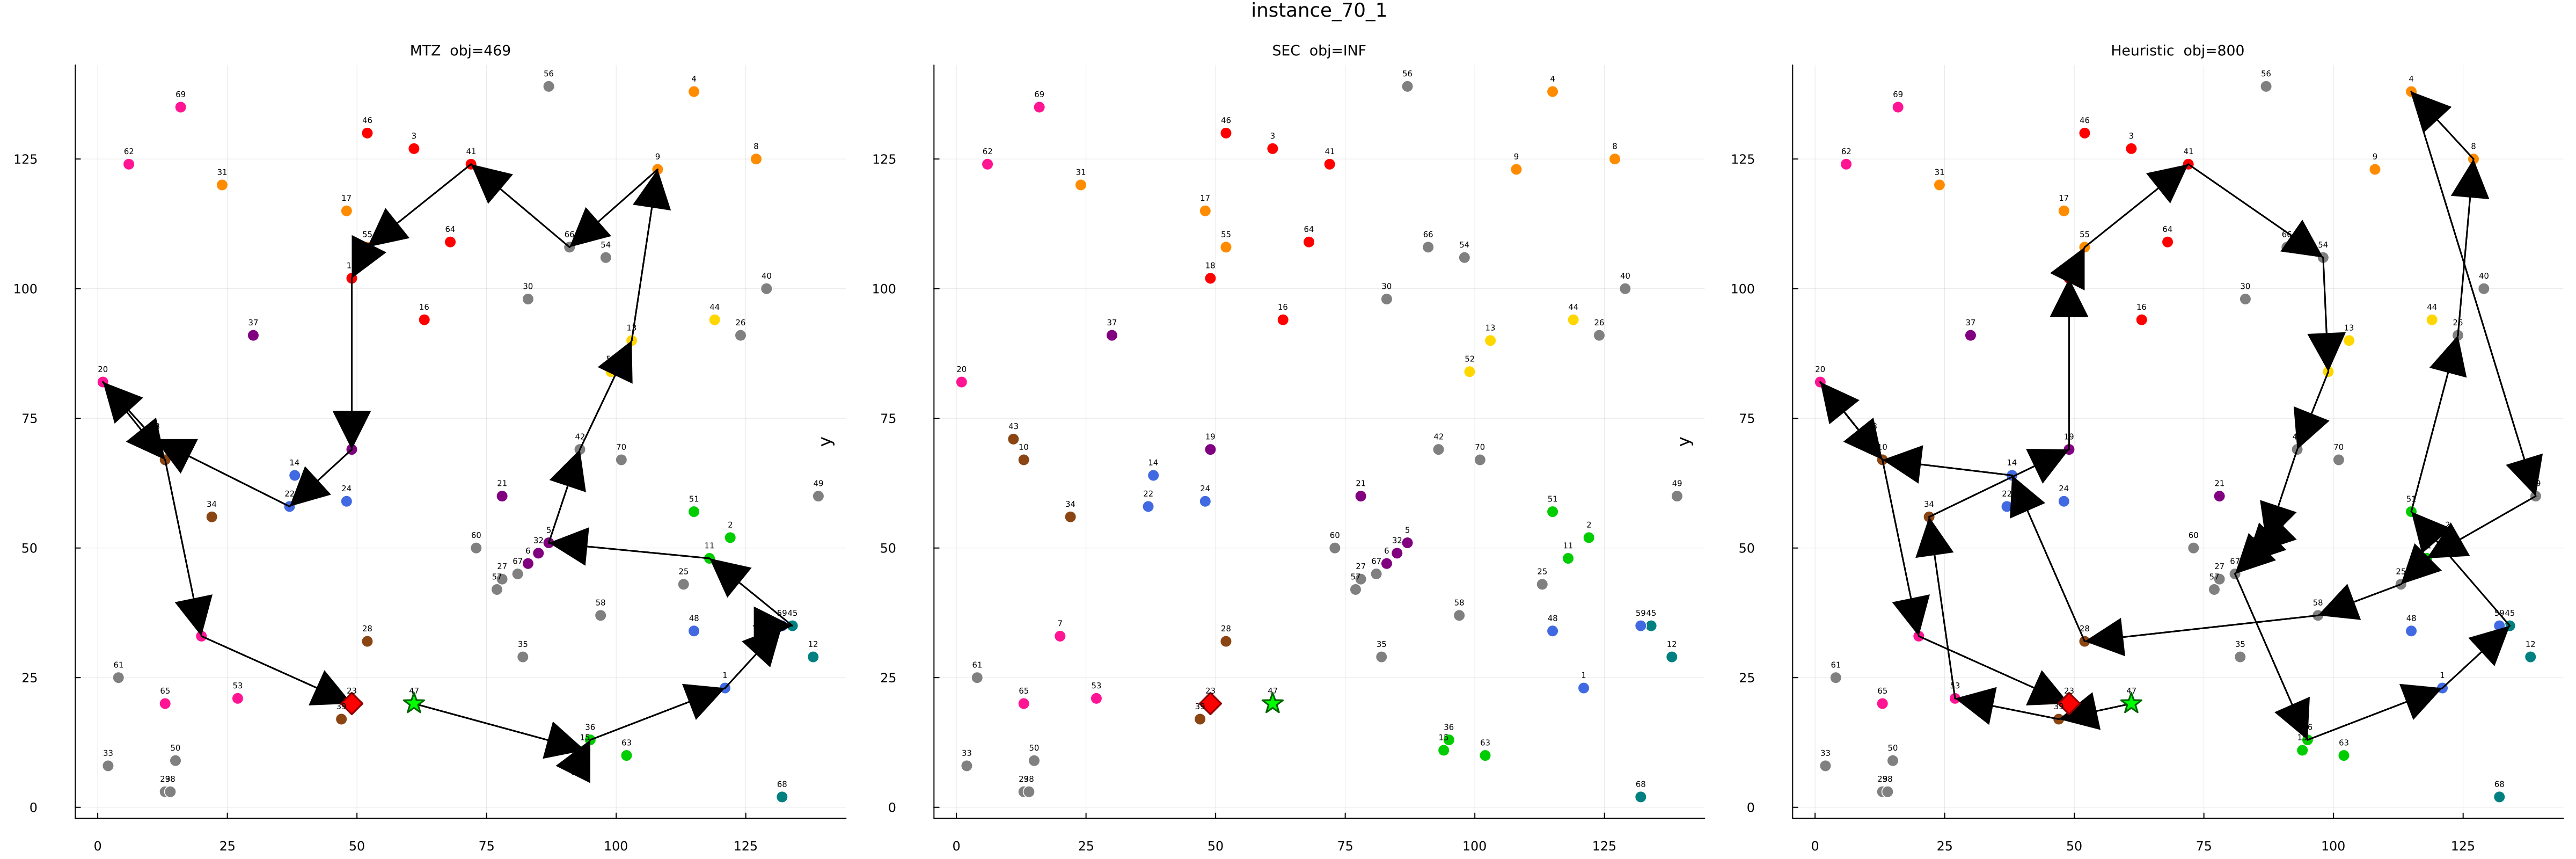
\includegraphics[width=\textwidth]{instance_70_1_results.png}
  \caption{Solution paths on \texttt{instance\_70\_1} ($n=70$, $m=16$). Both ILP
           models timed out; MTZ best incumbent cost~469.}
\end{figure}


%% ═════════════════════════════════════════════════════════════════════════════
\section{Analysis and Critical Discussion}
%% ═════════════════════════════════════════════════════════════════════════════

\subsection{MTZ vs.\ SEC: Theory Confirmed, Practice More Nuanced}

The theoretical prediction from the lectures is that SEC provides a tighter LP
relaxation ($z_{\mathrm{LP}}^{\mathrm{SEC}} \geq z_{\mathrm{LP}}^{\mathrm{MTZ}}$),
which translates to fewer B\&B nodes via the pruning-by-bound criterion. Our results
confirm the node count prediction consistently: SEC explores $37\times$ fewer nodes
than MTZ on \texttt{instance\_40\_1} (35 vs.\ 1\,295), $376\times$ fewer on
\texttt{instance\_20\_4} (379 vs.\ 142\,906), and $2.8\times$ fewer on the 70-node
instance (11\,647 vs.\ 32\,330).

However, wall-clock time tells a different story. The iterative SEC implementation
re-solves the ILP from scratch after each cut batch, discarding the B\&B tree each
time. This overhead means SEC solved only 1 of 7 custom instances within 120\,s,
while MTZ solved 5 of 7. The comparison is therefore \textbf{unfair to SEC}: we are
measuring implementation quality (iterative vs.\ lazy callbacks), not the intrinsic
strength of the formulation. A lazy-callback implementation would preserve the B\&B
tree across cuts and let the tighter LP bound directly reduce total work.

This is an important methodological limitation: our experimental conclusions about
SEC being ``slower'' apply only to the iterative variant, not to SEC in general.

\subsection{Integrality Gap and Bound Quality}

On instances where MTZ reached the time limit without proving optimality
(\texttt{instance\_80\_1}, \texttt{instance\_70\_1}), we can compute the
\textbf{optimality gap}: the relative distance between the best incumbent found
and the best LP lower bound at termination. Unfortunately HiGHS does not
expose the final LP bound directly through JuMP's interface, so we cannot report
the exact gap. This is a limitation of our reporting.

What we can observe is that on \texttt{instance\_80\_1}, MTZ explored 53\,334~nodes
in 120\,s without closing the gap. The large node count suggests the LP relaxation
is still loose at that scale. Adding valid inequalities --- such as the rounded
capacity constraints from the lecture on strengthening ILP formulations ---
or switching to the lazy-callback SEC would likely tighten the bound and reduce the
tree.

\subsection{Why the Heuristic Fails on Sparse Instances}

The greedy construction fails on \texttt{instance\_50\_1} ($R=28$) and
\texttt{instance\_70\_1} ($R=35$) by producing legs that exceed the range $R$.
Understanding \emph{why} matters more than simply labelling the solution ``invalid''.

The root cause is a mismatch between two phases. During the main greedy loop, the
algorithm calls Dijkstra to escape dead ends, returning a multi-hop sub-path. This
sub-path is range-feasible by construction (each hop $\leq R$). However, when the
sub-path passes through nodes that are already visited, those intermediate nodes are
skipped to avoid duplicates, \textbf{leaving a direct long-distance connection}
between two non-adjacent nodes in the sub-path. This connection was never checked
for range feasibility.

This is a structural bug: the heuristic confuses \emph{graph-theoretic path
feasibility} (each edge $\leq R$) with \emph{list connectivity} (adjacent entries
in the path vector). The fix is to either always include intermediate hops even if
they are revisited (allowing repeat visits), or to search explicitly for a
range-feasible escape that avoids already-visited nodes.

More broadly, greedy nearest-neighbour strategies are poorly suited to problems
where the range constraint creates a sparse graph. In a sparse graph, early greedy
choices can paint the algorithm into a corner from which no range-feasible escape
exists --- a situation that no amount of local search can recover from. A
better-suited construction for sparse instances would be to solve a \emph{shortest
path} problem on the range graph first (to find if $s \to t$ is even reachable),
then greedily insert region-covering detours along that backbone path.

\subsection{Limitations of the Models}

Both ILP models share a structural limitation: the \textbf{set-covering constraint
(C5)} does not interact with the flow constraints in any tightening way. It simply
requires $\sum_{i: r_i = k} y_i \geq 1$ independently of which arcs are used.
A stronger formulation would couple coverage to connectivity: if a region-covering
node $i$ is visited, it must be \emph{reachable} from $s$ along used arcs. This is
already enforced implicitly by the flow constraints (C3), but explicitly adding
cover-flow linking inequalities could tighten the LP relaxation further.

Another limitation is the absence of \textbf{symmetry breaking}. When multiple
optimal paths exist (e.g., same cost, different orderings of equivalent nodes), the
B\&B tree is enlarged unnecessarily. Standard symmetry-breaking constraints for
path problems would reduce this.

\subsection{Connections to Course Material}

The three approaches in this project connect directly to the lecture topics:
\begin{itemize}[nosep]
  \item \textbf{LP duality} (Cours~1): the LP relaxation gives a lower bound
        $z_{\mathrm{LP}} \leq z_{\mathrm{ILP}}^*$. Complementary slackness would
        identify which constraints are binding at the LP optimum and could guide
        cut selection.
  \item \textbf{Branch-and-bound} (Cours~2): both ILP models are solved by B\&B.
        The three pruning criteria (optimality, bound, infeasibility) are all active.
        The large node counts on medium instances suggest the LP bounds are still
        loose and better cuts or branching rules would help.
  \item \textbf{Cutting planes and separation} (Cours~3): the SEC model is a
        cutting-plane approach. The separation problem reduces to connected-component
        detection --- $O(n + |A|)$ per integer solution --- far simpler than the
        general max-flow separation for fractional solutions.
  \item \textbf{Lagrangian relaxation} (Cours~4): relaxing constraint~(C5) into the
        objective with multipliers $\lambda_k$ would decompose the problem into a
        shortest-path subproblem (flow + range) plus a penalty term. The Lagrangian
        bound $z_{\mathrm{LD}} \geq z_{\mathrm{LP}}^{\mathrm{MTZ}}$ could provide
        tighter bounds without the overhead of SEC.
\end{itemize}


%% ═════════════════════════════════════════════════════════════════════════════
\section{Conclusion}
%% ═════════════════════════════════════════════════════════════════════════════

We modelled the aerodrome race problem using two ILP formulations and a greedy
heuristic, and tested them on 10 instances ranging from $n = 6$ to $n = 80$.

The \textbf{MTZ model} is the practical winner in our setting: it proved optimality
on 7 of 9 instances within 120\,s, including all instances up to $n = 50$. Its
weaker LP bound is compensated by having no iterative overhead.

The \textbf{SEC model} consistently explores far fewer B\&B nodes, confirming the
theory. However, our iterative implementation pays a heavy restart cost at each cut
batch and proved optimality on only 2 of 9 instances. The conclusion is not that
SEC is inferior it is that \emph{iterative SEC is inferior to lazy-callback
SEC}. With HiGHS's support for generic callbacks or with Gurobi/CPLEX, a
lazy-callback implementation would be expected to outperform MTZ on all but the
smallest instances.

The \textbf{heuristic} succeeds on 7 of 9 instances with gaps of 5--14\% and
negligible running time. It fails on sparse instances ($R$ tight relative to the
coordinate domain) due to a structural mismatch in the escape mechanism. The
appropriate fix is to make the Dijkstra sub-path always preserve range feasibility
even when revisiting intermediate nodes.

%\paragraph{What we would do differently.}
%The most impactful improvement would be to implement SEC with proper lazy callbacks,
%which would make the comparison between MTZ and SEC meaningful. Beyond that:
%\begin{itemize}[nosep]
%  \item Use the heuristic solution as a \textbf{warm-start incumbent} for both ILP
%        models, reducing the initial optimality gap and enabling earlier pruning.
%  \item Add \textbf{Lagrangian relaxation} on the region-covering constraints
%        (Cours~4) as an alternative lower bound, which could be tighter than the MTZ
%        LP bound and cheaper to compute than SEC cuts.
%  \item For the heuristic, replace the greedy construction on sparse instances with
%        a \textbf{backbone approach}: first find the shortest $s \to t$ path on the
%        range graph (ensuring feasibility), then greedily insert region-covering
%        detours without breaking the backbone.
%\end{itemize}

\newpage

%% ─── Bibliography ────────────────────────────────────────────────────────────
\bibliographystyle{plain}
\bibliography{references}

\end{document}